\chapter{Newtonian Gravity, Free Fall, and Gauss's Theorem}

\section{Why Begin General Relativity with Newton?}

Gravity is unlike the electric and magnetic forces. Its deepest formulation
is tied to the geometry of space and time, and that connection is the subject
of general relativity. We shall not begin there. We shall begin with
Newtonian gravity, but arrange the old theory so that the ideas needed later
are already visible.

The natural starting point is an inertial frame: a set of spatial coordinates
and clocks in which a force-free test body moves with constant velocity. In
such a frame Newton's equation is
\begin{equation}
  \vec F=m\vec a.
  \label{eq:l01-newton}
\end{equation}
The force and acceleration are three-vectors; the mass is a scalar. In
components,
\begin{equation}
  F_i=ma_i=m\ddot x_i,
  \qquad i=1,2,3.
  \label{eq:l01-newton-components}
\end{equation}

\begin{figure}[tbp]
  \centering
  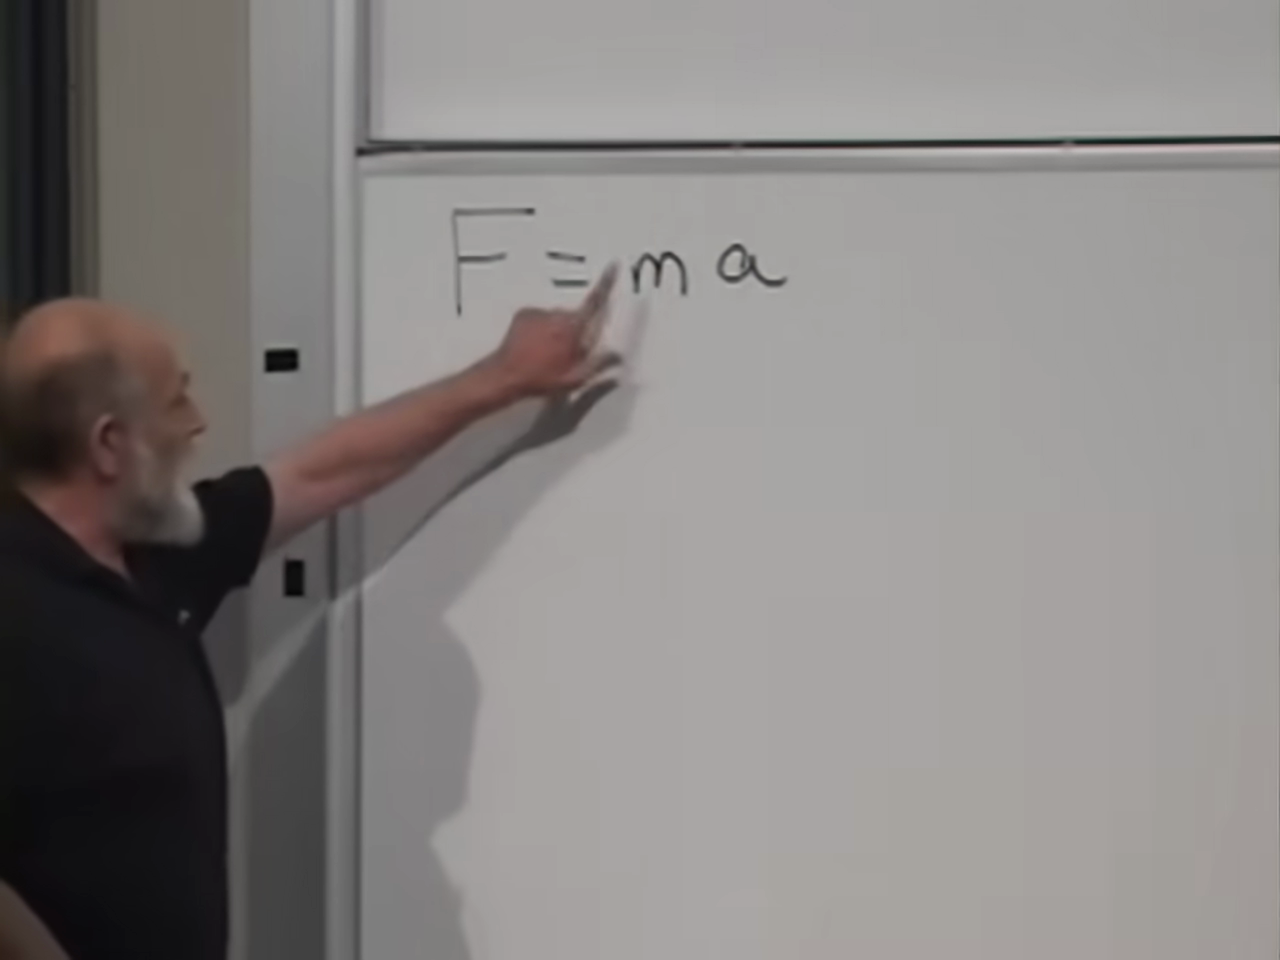
\includegraphics[width=0.68\textwidth]{lecture_01_figure_01.png}
  \caption{Newton's law is introduced before gravity is specialized. The
  spoken discussion immediately interprets the board equation as a
  three-vector relation.}
  \lectureframe{00:03:45}
\end{figure}

A particle's coordinates \(x_1,x_2,x_3\) are the components of its position
vector \(\vec r\). Their first and second time derivatives are the components
of velocity and acceleration:
\begin{equation}
  \vec v=\dot{\vec r},
  \qquad
  \vec a=\ddot{\vec r}.
  \label{eq:l01-kinematics}
\end{equation}
In Newtonian mechanics mass is conserved. A cup becomes lighter when coffee
is removed, but that is transport of matter, not spontaneous loss of mass.
These elementary distinctions will matter because gravity places the same
mass on both sides of Equation~\eqref{eq:l01-newton}.

\section{Galileo's Uniform Gravitational Field}

Before using Newton's inverse-square law, take the approximation appropriate
to experiments near the Earth's surface. Over a sufficiently small region
the Earth may be treated as flat. Then \emph{down} has the same direction
everywhere, and the strength of gravity may be treated as independent of
height. If \(x_2\) points upward, the vertical force is
\begin{equation}
  F_2=-mg.
  \label{eq:l01-flat-force}
\end{equation}
Here \(g\) is approximately \(9.8\,\mathrm{m\,s^{-2}}\) at the Earth's
surface. It differs on the Moon or Jupiter because it depends on the source,
but it does not depend on the mass of the body being dropped.

Combining Equations~\eqref{eq:l01-newton-components} and
\eqref{eq:l01-flat-force},
\begin{align}
  m\ddot x_2&=-mg,\\
  \boxed{\ddot x_2=-g.}
  \label{eq:l01-mass-cancels}
\end{align}

\begin{figure}[tbp]
  \centering
  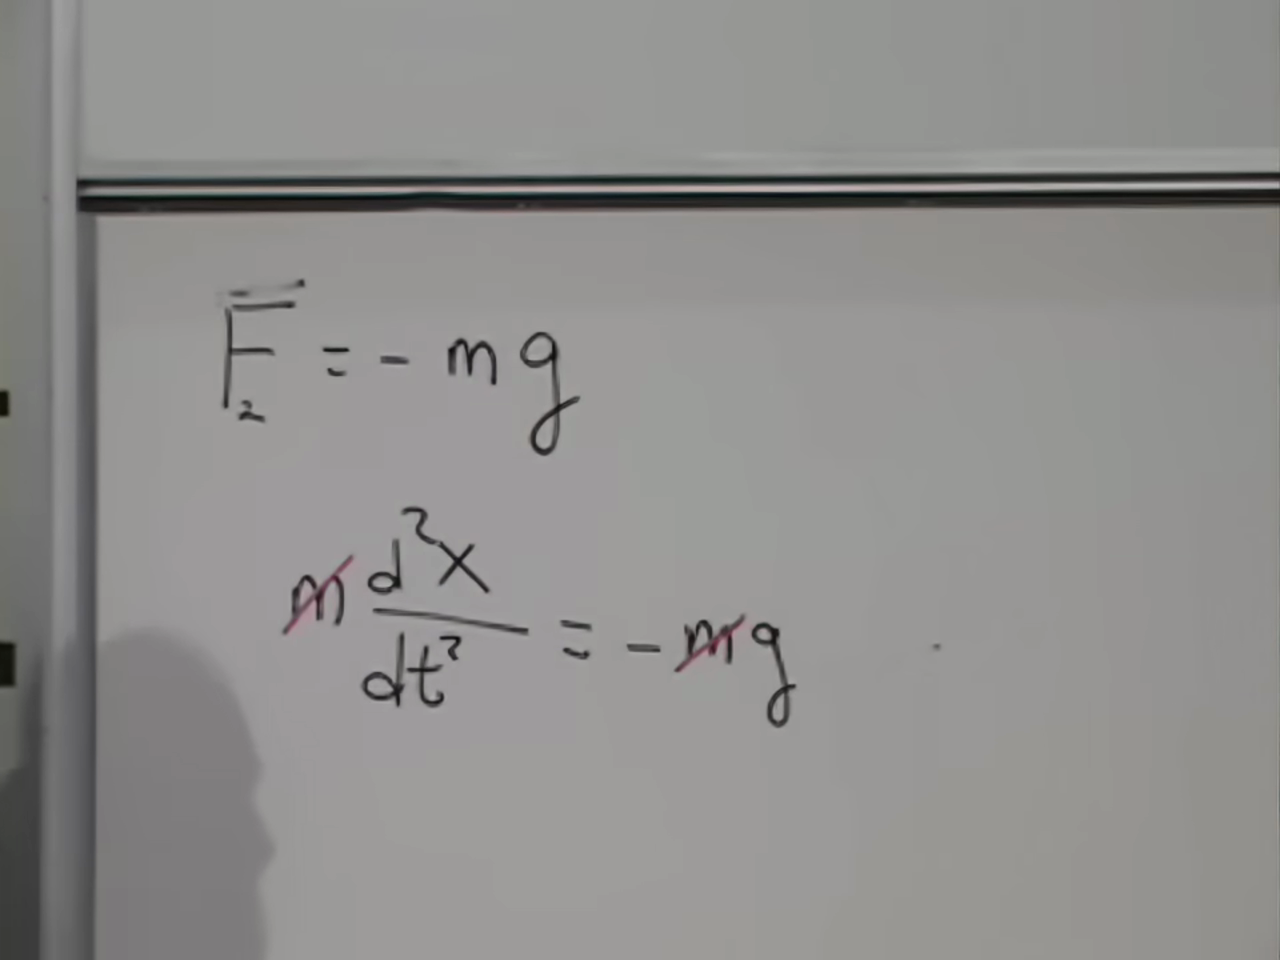
\includegraphics[width=0.70\textwidth]{lecture_01_figure_02.png}
  \caption{Galileo's near-surface law and the cancellation of the falling
  body's mass from its equation of motion.}
  \lectureframe{00:12:40}
\end{figure}

This cancellation is gravity's special feature. An electric force is
proportional to charge, while inertia is proportional to mass; charged and
uncharged objects therefore respond differently to an electric field. In
gravity the coupling and the inertia are proportional to the same quantity.
Absent air resistance, a cannonball and a feather obey the same trajectory.
Whether Galileo actually dropped objects from the Leaning Tower of Pisa is
less important than the content of the experiment; inclined-plane
measurements already expose the same universal acceleration.

\section{Free Fall and the First Equivalence Principle}

The cancellation has a stronger consequence than equal fall times. Imagine
a diffuse cloud of noninteracting particles released from rest. The
particles may have different masses and sizes and may begin at different
heights. In a uniform field each obeys
\(\ddot{\vec r}_a=\vec g_0\), so for any pair,
\begin{equation}
  \frac{d^2}{dt^2}
  \left(\vec r_a-\vec r_b\right)=0.
  \label{eq:l01-relative-cloud}
\end{equation}
If their initial relative velocities vanish, their separations remain
fixed. The cloud translates without changing shape.

\begin{figure}[tbp]
  \centering
  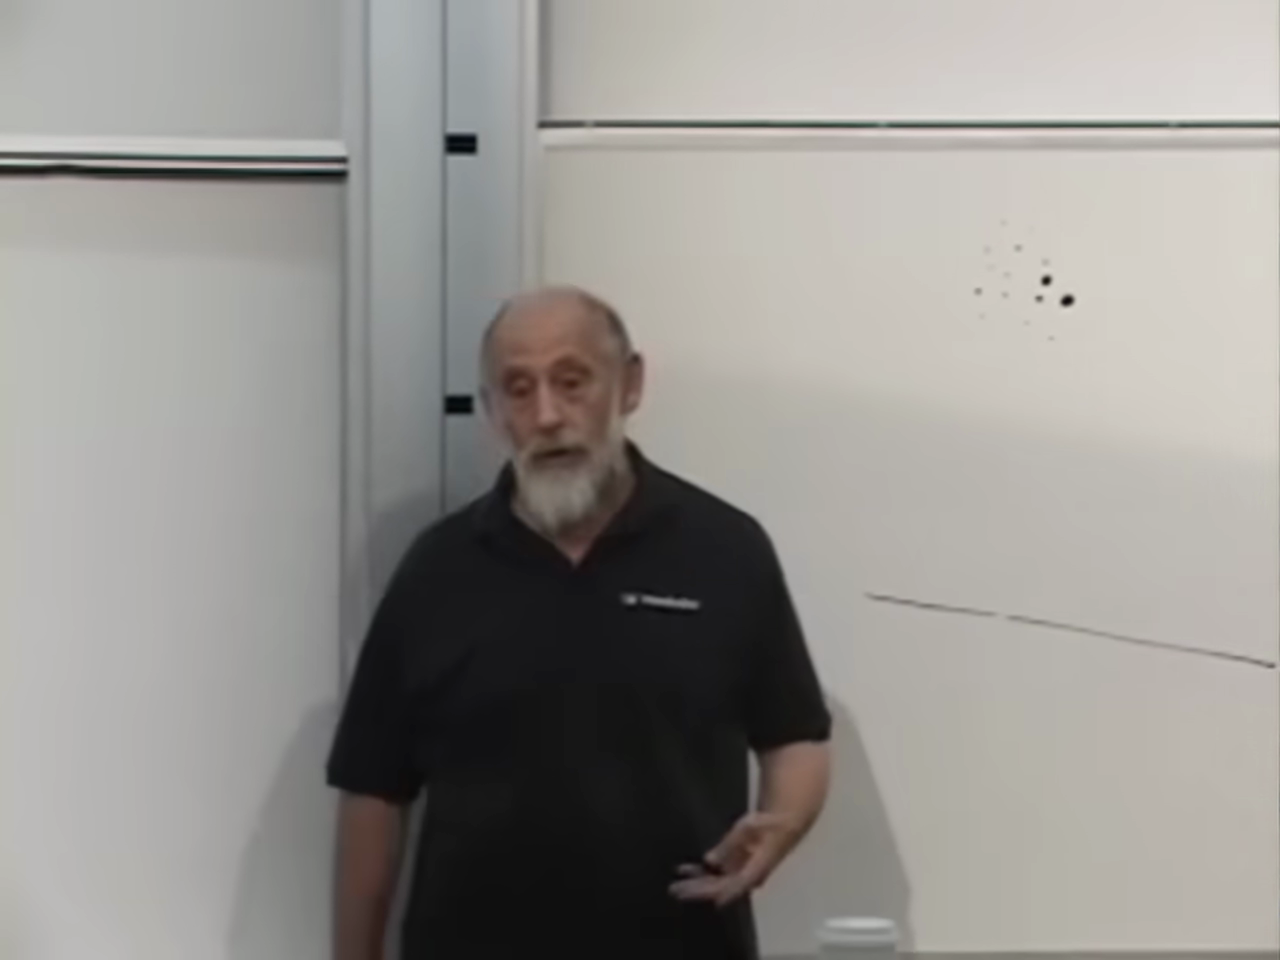
\includegraphics[width=0.66\textwidth]{lecture_01_figure_03.png}
  \caption{A loose cloud of particles used to make universality of free fall
  into a statement about relative motion and internal stress.}
  \lectureframe{00:17:00}
\end{figure}

Even if struts held the particles together, the struts would carry no
gravity-induced stress in this approximation: every part wants to make the
same motion. A self-contained freely falling laboratory is therefore
mechanically indistinguishable from an inertial laboratory far from all
gravitating bodies. This is the first form of the equivalence principle.

\begin{classroomqa}
\audiencequestion{Could the falling cloud detect gravity optically, perhaps
by measuring laser distances between its particles?
\lecturetimestamp{00:17:30--00:20:16}}
\lecturerresponse{Not in a perfectly uniform field. The relative positions
of freely falling particles do not change, so internal optical measurements
give the same result as they would in gravity-free inertial motion. Looking
at the floor would reveal motion relative to an external supported object,
but that is no longer a self-contained experiment. The floor fails to fall
only because other forces support it.}
\end{classroomqa}

\begin{classroomqa}
\audiencequestion{Surely we can feel when we are accelerating. Does the
peculiar sensation of stepping from a high building reveal gravity?
\lecturetimestamp{00:20:17--00:22:44}}
\lecturerresponse{What the body ordinarily feels is the support force that
prevents free fall: pressure on the feet, the chair, and the internal forces
transmitting that pressure. Remove the support and those forces disappear.
The resulting sensation would be the same in a freely drifting spacecraft
far from gravitating bodies. In this precise sense we feel \emph{not
falling}, rather than uniform free fall itself.}
\end{classroomqa}

The qualification \emph{uniform} is essential. A real planet is finite and
round. Its field changes with position, and those changes will soon restore
an observable effect through tidal forces.

\section{Newton's Inverse-Square Law}

Move now beyond the flat-Earth approximation. Every mass attracts every
other mass. For two bodies of masses \(m\) and \(M\), separated by a distance
\(r\), the magnitude of either force is
\begin{equation}
  F=\frac{GmM}{r^2},
  \label{eq:l01-scalar-gravity}
\end{equation}
where
\begin{equation}
  G\simeq 6.67\times10^{-11}\,
  \mathrm{N\,m^2\,kg^{-2}}.
  \label{eq:l01-G}
\end{equation}
The constant is needed dimensionally, and its small numerical value records
the weakness of gravity on laboratory scales. Two one-kilogram masses one
meter apart attract with only about
\(6.67\times10^{-11}\,\mathrm N\). A rubbed, electrically charged object or
a small magnet produces a readily visible deflection where even a nearby
heavy mass does not. Gravity dominates our weight because the Earth supplies
an enormous source mass.

\begin{classroomqa}
\audiencequestion{If the two forces are equal and opposite, why does a
falling object accelerate noticeably while the Earth hardly moves?
\lecturetimestamp{00:27:07--00:29:02}}
\lecturerresponse{Newton's third law equates the forces, not the
accelerations. Since \(\vec a=\vec F/m\), the same force gives the enormous
Earth an imperceptibly small acceleration and gives the much lighter object
a much larger one. Both bodies actually move about their common center of
mass.}
\end{classroomqa}

\subsection{Kepler's Clue}

Newton did not obtain the inverse-square dependence from dimensional
analysis. Kepler's planetary laws supplied the decisive clue. For a circular
orbit of radius \(r\) and angular frequency \(\omega\),
\begin{equation}
  a_{\mathrm{circ}}=\omega^2r.
  \label{eq:l01-centripetal}
\end{equation}
If the acceleration caused by gravity varies as \(1/r^2\), then
\begin{equation}
  \omega^2r\propto\frac1{r^2}
  \quad\Longrightarrow\quad
  \omega^2\propto\frac1{r^3}.
\end{equation}
Since \(T=2\pi/\omega\),
\begin{equation}
  \boxed{T^2\propto r^3,}
  \label{eq:l01-kepler-third}
\end{equation}
which is Kepler's period--radius law. The same inverse-square force also
produces elliptical, not merely circular, bound orbits.

\begin{classroomqa}
\audiencequestion{What happens as the two objects approach one another or
touch? Does the inverse-square law diverge?
\lecturetimestamp{00:32:32--00:34:37}}
\lecturerresponse{The Newtonian point-particle expression is not a complete
short-distance theory of matter. Once extended bodies touch, electrostatic,
atomic, and nuclear forces become important. The contact force supporting an
eraser on a table is itself largely electromagnetic. Newton's law remains
the long-range gravitational contribution, not the only interaction.}
\end{classroomqa}

This comparison also sharpens the universality of gravity. Electric fields
distinguish charge from neutrality and can attract or repel. Newtonian
gravity acts on every mass and is always attractive.

\section{Direction and the Many-Body Law}

Equation~\eqref{eq:l01-scalar-gravity} gives only a magnitude. Put \(M\) at
the origin and let \(\vec r\) point from \(M\) to \(m\). Attraction makes the
force point opposite to \(\vec r\):
\begin{equation}
  \vec F
  =-\frac{GmM}{r^2}\hat{\vec r}
  =-\frac{GmM}{r^3}\vec r,
  \qquad
  \hat{\vec r}=\frac{\vec r}{r}.
  \label{eq:l01-vector-gravity}
\end{equation}
The extra \(r\) in the denominator compensates for the magnitude of the
vector inserted in the numerator.

\begin{figure}[tbp]
  \centering
  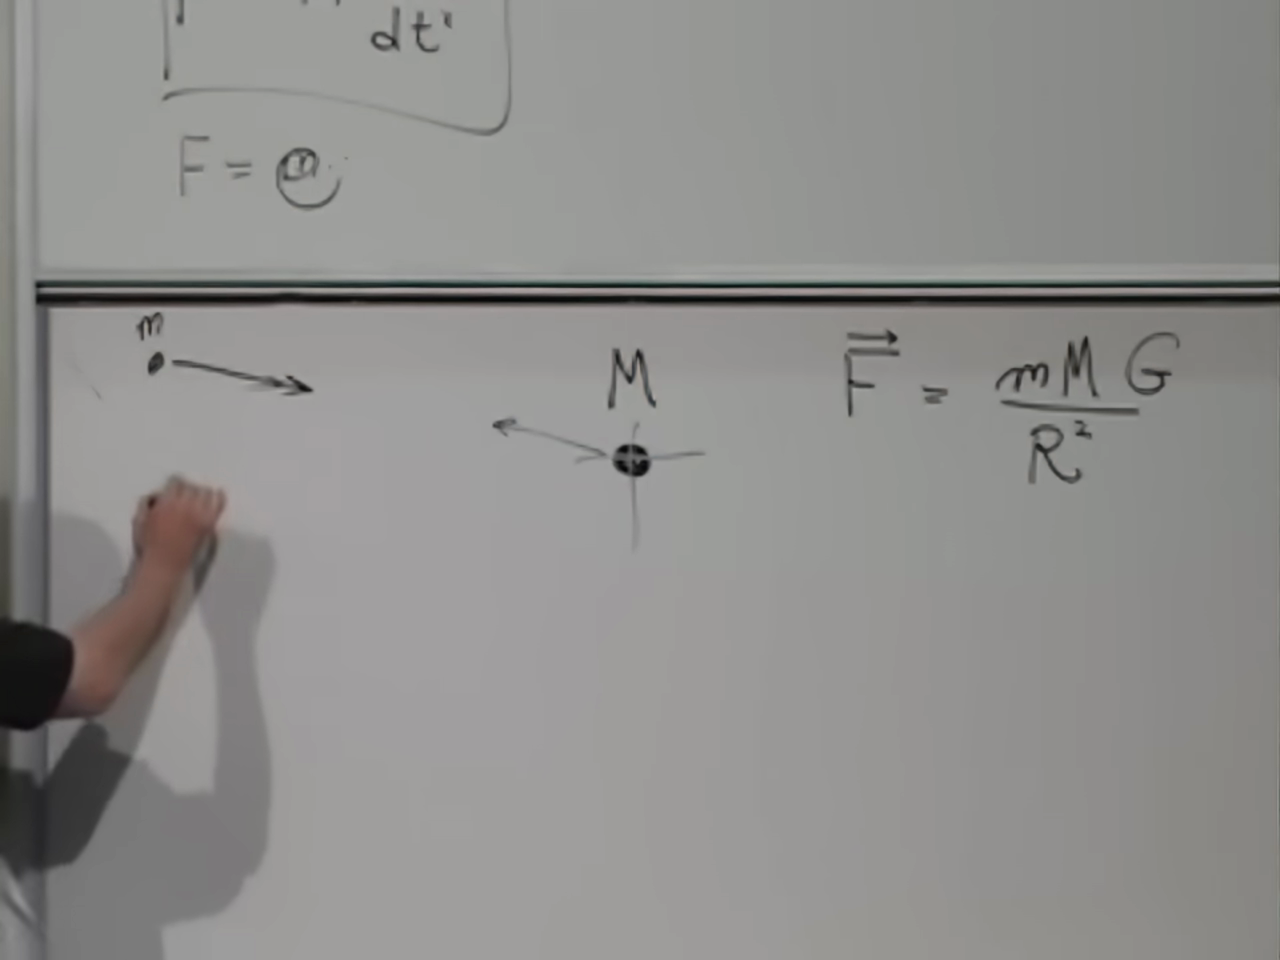
\includegraphics[width=0.78\textwidth]{lecture_01_figure_04.png}
  \caption{The scalar inverse-square law and the source-to-particle geometry
  from which its vector direction is fixed.}
  \lectureframe{00:36:25}
\end{figure}

For many particles, let \(\vec r_i\) and \(m_i\) be the position and mass of
particle \(i\). Define
\(\vec r_{ij}=\vec r_j-\vec r_i\), the vector pointing from \(i\) to \(j\).
The force on \(i\) is then
\begin{equation}
  \vec F_i
  =
  \sum_{j\ne i}
  Gm_im_j
  \frac{\vec r_j-\vec r_i}
       {|\vec r_j-\vec r_i|^3}.
  \label{eq:l01-many-body-force}
\end{equation}
Every term points toward its source. The lecture's temporary minus-sign
confusion is only a choice between
\(\vec r_{ij}\) and \(\vec r_{ji}=-\vec r_{ij}\); once the displacement
vector is defined, the sign is fixed.

\begin{figure}[tbp]
  \centering
  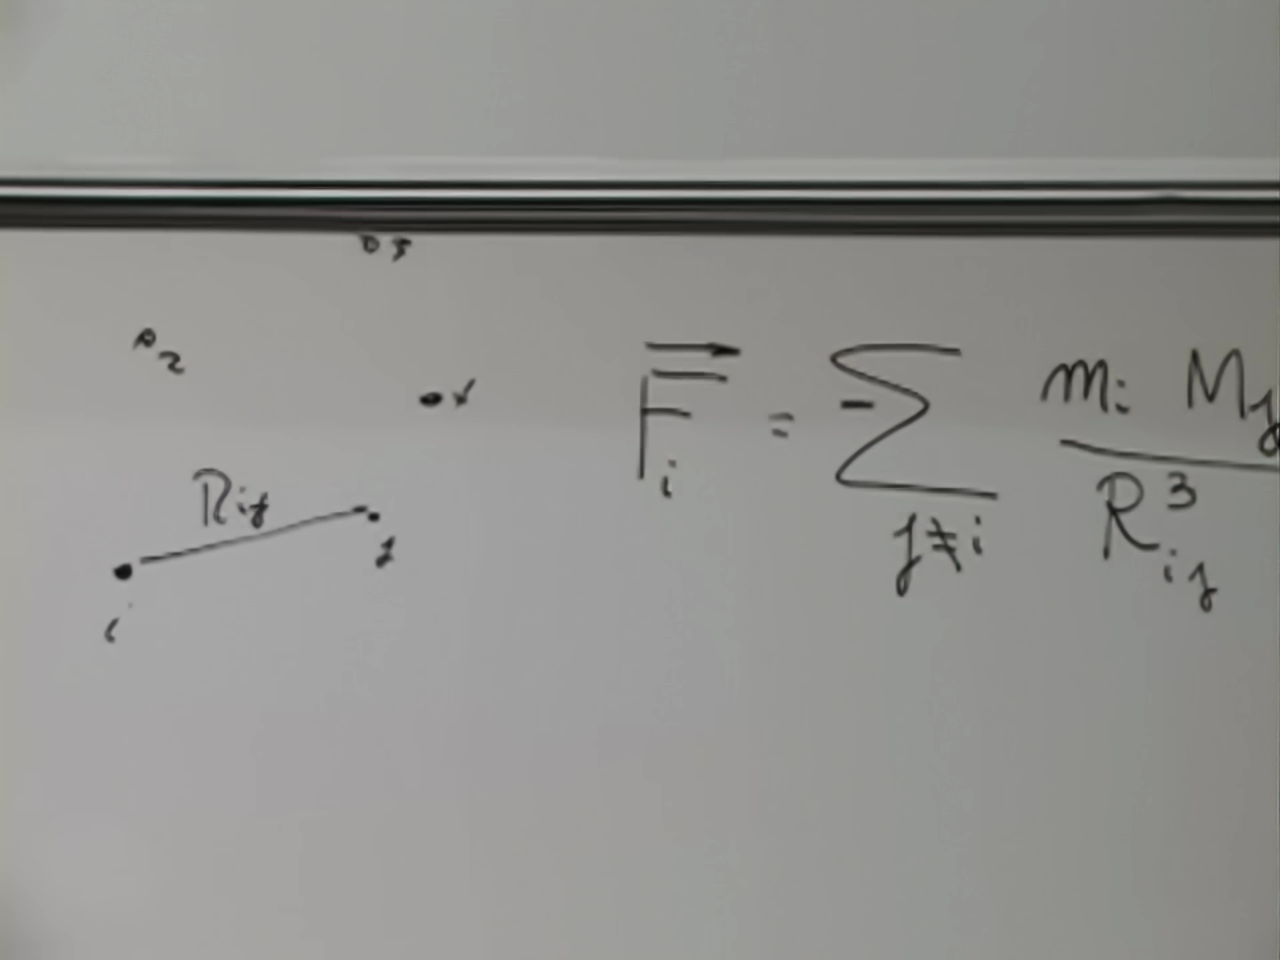
\includegraphics[width=0.80\textwidth]{lecture_01_figure_05.png}
  \caption{The many-body force sum together with the displacement-vector
  convention. This unobstructed frame precedes the live sign correction.}
  \lectureframe{00:40:40}
\end{figure}

Substitution into \(m_i\vec a_i=\vec F_i\) cancels the mass of the body whose
motion is being followed:
\begin{equation}
  \boxed{
  \vec a_i
  =
  \sum_{j\ne i}
  Gm_j
  \frac{\vec r_j-\vec r_i}
       {|\vec r_j-\vec r_i|^3}.}
  \label{eq:l01-many-body-acceleration}
\end{equation}
The acceleration depends on all the source masses but not on \(m_i\).
Universality of free fall survives the move from uniform gravity to the full
Newtonian field.

\begin{classroomqa}
\audiencequestion{Once all the masses move, does every particle retain one
uniform acceleration, perhaps toward the center of the whole system?
\lecturetimestamp{00:43:28--00:46:43}}
\lecturerresponse{No. Equation~\eqref{eq:l01-many-body-acceleration} gives
the instantaneous acceleration from the instantaneous positions. As the
positions change, so do the magnitudes and directions of all terms. Bodies
may even be moving apart while their accelerations point toward one another.
Solving the coupled equations is a nonlinear many-body problem; superposition
of instantaneous forces does not make the trajectories linear or uniform.}
\end{classroomqa}

\section{Tidal Forces: Where Uniform Free Fall Fails}

A realistic gravitational field varies across an extended object. Imagine a
person thousands of miles tall falling feet first toward the Earth. The feet
are closer to the source and accelerate more strongly than the head, so the
body stretches radially. Turn the person sideways. The forces on the two ends
point along slightly different radii toward the Earth's center, so the body
is compressed transversely.

\begin{figure}[tbp]
  \centering
  
\includegraphics[width=0.66\textwidth]{lecture_01_figure_06.png}
  \caption{The board's extended-body sketches: radial variation stretches a
  vertical body, while converging field directions compress it
  transversely.}
  \lectureframe{00:48:00}
\end{figure}

For two nearby points separated by \(\delta\vec x\),
\begin{equation}
  \delta g_i
  =
  g_i(\vec x+\delta\vec x)-g_i(\vec x)
  \simeq
  \frac{\partial g_i}{\partial x_j}\,\delta x_j.
  \label{eq:l01-tidal-gradient}
\end{equation}
Thus a freely falling laboratory removes the common acceleration
\(\vec g(\vec x)\), but not its spatial gradient. For a point source,
\begin{equation}
  \vec g(\vec r)=-\frac{GM}{r^3}\vec r.
\end{equation}
The radial eigenvalue of its gradient is \(2GM/r^3\), while each transverse
eigenvalue is \(-GM/r^3\): stretching in one direction is accompanied by
compression in the other two.

These are tidal forces. The Moon's field is slightly stronger on the near
side of the Earth and slightly weaker on the far side. The solid Earth
resists deformation, while the oceans respond more visibly, producing
approximately opposite tidal bulges. The effect becomes negligible only
when the falling system is small compared with the length scale over which
the field changes.

\begin{classroomqa}
\audiencequestion{Did Newton understand the lunar origin of the tides?
\lecturetimestamp{00:50:29--00:51:09}}
\lecturerresponse{He understood the essential tidal mechanism, although the
lecture does not settle how accurately he calculated the ocean's actual
deformation. The point needed here is the differential pull: a finite body
samples different values and directions of the Moon's field.}
\end{classroomqa}

\section{The Gravitational Field}

The many-body formula suggests a cleaner description. Add an imagined test
particle so light that it does not disturb the sources. Place it at
\(\vec x\) and observe its acceleration. The gravitational field is that
acceleration:
\begin{equation}
  \vec g(\vec x,t)
  \equiv
  \frac{\vec F_{\mathrm{test}}}{m_{\mathrm{test}}}.
  \label{eq:l01-field-definition}
\end{equation}
Because the test mass cancels, the result is independent of which test
particle is used. If source masses \(m_j\) occupy positions \(\vec r_j(t)\),
\begin{equation}
  \boxed{
  \vec g(\vec x,t)
  =
  \sum_j Gm_j
  \frac{\vec r_j(t)-\vec x}
       {|\vec r_j(t)-\vec x|^3}.}
  \label{eq:l01-field-sum}
\end{equation}
It is a vector at every point in space and, when the sources move, a function
of time as well.

\begin{figure}[tbp]
  \centering
  
\includegraphics[width=0.80\textwidth]{lecture_01_figure_07.png}
  \caption{The test-particle acceleration emerges from the many-body force
  law after the test mass is canceled.}
  \lectureframe{01:00:00}
\end{figure}

\begin{classroomqa}
\audiencequestion{In a whole ensemble, do sign choices or mutual influence
add some extra nonlinear term to the field formula?
\lecturetimestamp{00:52:36--00:56:09}}
\lecturerresponse{At a specified instant the force is exactly the vector sum
in Equation~\eqref{eq:l01-many-body-force}; attraction is already encoded by
the direction \(\vec r_j-\vec r_i\). Mutual influence enters when the
positions are evolved, because each trajectory changes the future field
seen by every other body. It complicates the solution, not the instantaneous
force law.}
\end{classroomqa}

\section{Divergence: Measuring Local Sources and Sinks}

After the break we need one piece of vector calculus. For a generic vector
field
\(\vec A=(A_x,A_y,A_z)\), define
\begin{equation}
  \boxed{
  \nabla\cdot\vec A
  =
  \frac{\partial A_x}{\partial x}
  +\frac{\partial A_y}{\partial y}
  +\frac{\partial A_z}{\partial z}.}
  \label{eq:l01-divergence}
\end{equation}
The upside-down triangle, \(\nabla\), represents the three spatial
derivatives. Although it acts on a vector field, the dot product leaves a
scalar.

\begin{figure}[tbp]
  \centering
  
\includegraphics[width=0.84\textwidth]{lecture_01_figure_08.png}
  \caption{The component definition of divergence. The arrows over
  \(\nabla\) and \(A\) matter: their dot product is a scalar.}
  \lectureframe{01:08:10}
\end{figure}

The name is easiest to understand through flow. Imagine a shallow lake of
fixed depth filled with incompressible water. If water is pumped in from
below, the horizontal velocity field spreads outward and has positive
divergence. If water is removed through a hidden drain, the arrows converge
and the divergence is negative. Uniform translation of the whole lake has
zero divergence even though the water is moving.

The local test is to draw a small boundary. If more water leaves than enters,
some water must have been supplied inside. In one dimension the same idea is
visible when rightward arrows grow longer as \(x\) increases:
\(\partial A_x/\partial x>0\).

\begin{figure}[tbp]
  \centering
  
\includegraphics[width=0.74\textwidth]{lecture_01_figure_09.png}
  \caption{The arrow field used to compare inflow and outflow across a small
  imagined control region. Longer outgoing arrows indicate positive local
  divergence.}
  \lectureframe{01:13:00}
\end{figure}

\begin{classroomqa}
\audiencequestion{Could the arrows spread because a compressible fluid is
thinning rather than because water is being pumped in?
\lecturetimestamp{01:12:18--01:14:45}}
\lecturerresponse{Yes. For a compressible fluid, velocity divergence can
change density instead of representing an external source. The lake analogy
deliberately fixes both density and depth so that velocity divergence may be
read directly as injected or removed water. The mathematical definition of
divergence itself does not depend on that simplifying interpretation.}
\end{classroomqa}

\section{Gauss's Theorem}

Let \(V\) be any volume with closed boundary \(\partial V\) and outward unit
normal \(\hat n\). Gauss's theorem states
\begin{equation}
  \boxed{
  \int_V(\nabla\cdot\vec A)\,d^3x
  =
  \oint_{\partial V}\vec A\cdot\hat n\,d\sigma.}
  \label{eq:l01-gauss}
\end{equation}
The left side adds all local sources and sinks in the interior. The right
side adds the net outward flux through the boundary. A tangential component
does not cross the boundary and therefore contributes nothing.

\begin{figure}[tbp]
  \centering
  
\includegraphics[width=0.82\textwidth]{lecture_01_figure_10.png}
  \caption{Gauss's theorem on the board: the volume integral of divergence
  equals the surface integral of the normal field component.}
  \lectureframe{01:20:30}
\end{figure}

\begin{classroomqa}
\audiencequestion{If no water is created, should the integrated divergence
always vanish?
\lecturetimestamp{01:20:37--01:22:33}}
\lecturerresponse{For an incompressible flow with no sources or sinks inside
the chosen region, yes: its net outward flux is zero. Water may still enter
one part of the boundary and leave another. A pump supplies positive
divergence; a drain supplies negative divergence. In the two-dimensional
lake the interior area integral equals a line integral around the boundary;
in three dimensions it becomes Equation~\eqref{eq:l01-gauss}.}
\end{classroomqa}

\section{Spherical Symmetry and the Inverse-Square Field}

Suppose \(\nabla\cdot\vec A\) is confined to a finite spherically symmetric
region. Surround it by a larger sphere of radius \(r\), and define the total
source strength
\begin{equation}
  Q=\int_V(\nabla\cdot\vec A)\,d^3x.
  \label{eq:l01-Q}
\end{equation}
As long as the Gaussian sphere encloses the source, \(Q\) is independent of
its radius. Spherical symmetry requires the exterior field to be radial and
to have the same magnitude at every point on the sphere. Therefore
\begin{align}
  Q
  &=
  \oint_{\partial V}\vec A\cdot\hat n\,d\sigma\\
  &=
  A(r)\,4\pi r^2,
\end{align}
and hence
\begin{equation}
  \boxed{
  \vec A(r)=\frac{Q}{4\pi r^2}\hat{\vec r}.}
  \label{eq:l01-spherical-field}
\end{equation}
The surface area is \(4\pi r^2\); the transient phrase
\emph{four-thirds} in the spoken calculation is immediately corrected on
the board.

\begin{figure}[tbp]
  \centering
  
\includegraphics[width=0.84\textwidth]{lecture_01_figure_11.png}
  \caption{Spherical symmetry turns Gauss's theorem into
  \(4\pi r^2A(r)=Q\), forcing an inverse-square radial field.}
  \lectureframe{01:28:30}
\end{figure}

\begin{classroomqa}
\audiencequestion{The result is written as a scalar magnitude. How is the
vector direction restored?
\lecturetimestamp{01:27:43--01:29:12}}
\lecturerresponse{Spherical symmetry supplies it. For positive divergence
the field is radial and outward, so multiplying the magnitude by
\(\hat{\vec r}\) gives Equation~\eqref{eq:l01-spherical-field}. For gravity
the field points inward, and the sign is reversed.}
\end{classroomqa}

Gravity is therefore analogous not to water emitted from a source but to
incompressible flow drawn into a sink. In continuum notation the precise
Newtonian statement is
\begin{equation}
  \nabla\cdot\vec g=-4\pi G\rho,
  \label{eq:l01-poisson-divergence}
\end{equation}
so for enclosed mass
\(M_{\mathrm{enc}}=\int_V\rho\,d^3x\),
\begin{equation}
  \oint_{\partial V}\vec g\cdot\hat n\,d\sigma
  =-4\pi G M_{\mathrm{enc}}.
  \label{eq:l01-gravity-gauss}
\end{equation}
For a point mass or any spherical source observed from outside,
\begin{equation}
  \vec g(r)=-\frac{GM}{r^2}\hat{\vec r}.
  \label{eq:l01-exterior-field}
\end{equation}
The fluid picture is only a mathematical analogy; it does not assert that
space is literally flowing.

\section{Newton's Shell Theorem}

The derivation used only spherical symmetry and total enclosed source. It
did not use the detailed radial density profile. We have therefore proved
Newton's theorem:

\begin{theorem}[Newton's shell theorem]
Outside any spherically symmetric mass distribution, the gravitational field
is exactly the field of a point mass with the same total mass placed at the
center. Inside a spherical shell of matter, the gravitational field
vanishes.
\end{theorem}

The exterior statement makes planetary gravity tractable. A spherical Earth
may be treated as though all its mass were at the center, provided the field
point lies outside the material. This special simplification belongs to the
inverse-square law; a generic \(1/r^n\) force would not reproduce it.

The restriction to exterior points matters. In a mine shaft through a
uniform-density Earth, a Gaussian sphere of radius \(r<R\) encloses only
\begin{equation}
  M_{\mathrm{enc}}(r)=\frac{4\pi}{3}\rho r^3.
\end{equation}
Consequently
\begin{equation}
  \vec g(r)
  =
  -\frac{GM_{\mathrm{enc}}(r)}{r^2}\hat{\vec r}
  =
  -\frac{4\pi G\rho}{3}\,\vec r.
  \label{eq:l01-inside-uniform-sphere}
\end{equation}
The field becomes small near the center and vanishes at the center itself;
it is not the divergent field obtained by concentrating the entire Earth
there.

\begin{figure}[tbp]
  \centering
  
\includegraphics[width=0.76\textwidth]{lecture_01_figure_12.png}
  \caption{The hollow-shell discussion. Outside, the shell acts like a point
  mass at the center; inside, spherical symmetry and zero enclosed mass give
  zero field.}
  \lectureframe{01:37:10}
\end{figure}

\begin{classroomqa}
\audiencequestion{Inside a hollow shell, should the nearer wall not pull more
strongly than the farther wall?
\lecturetimestamp{01:35:30--01:38:04}}
\lecturerresponse{Individual nearby elements do pull more strongly, but
there is less nearby area subtending a given solid angle; the larger amount
of farther material cancels that advantage exactly. Gauss's theorem packages
the cancellation. A centered Gaussian sphere encloses no mass, and spherical
symmetry makes the radial field constant over it, so
\(4\pi r^2g(r)=0\) and therefore \(\vec g=0\) everywhere in the cavity.}
\end{classroomqa}

General relativity has a corresponding exterior result: a spherically
symmetric vacuum field is fixed by the total mass and has the Schwarzschild
form, the same exterior geometry associated with a nonrotating black hole.
That theorem lies ahead. For now the essential lesson is already visible in
Newtonian language: universal free fall shifts attention from force to
acceleration, spatial variation appears as tides, and Gauss's theorem turns
local source information into the global field.
